%!TEX root = ../../report.tex
\section{Mapping an industrial environment}
\label{mapping_simulation}

\begin{figure}
	\centering
	\begin{subfigure}[b]{0.45\textwidth}
		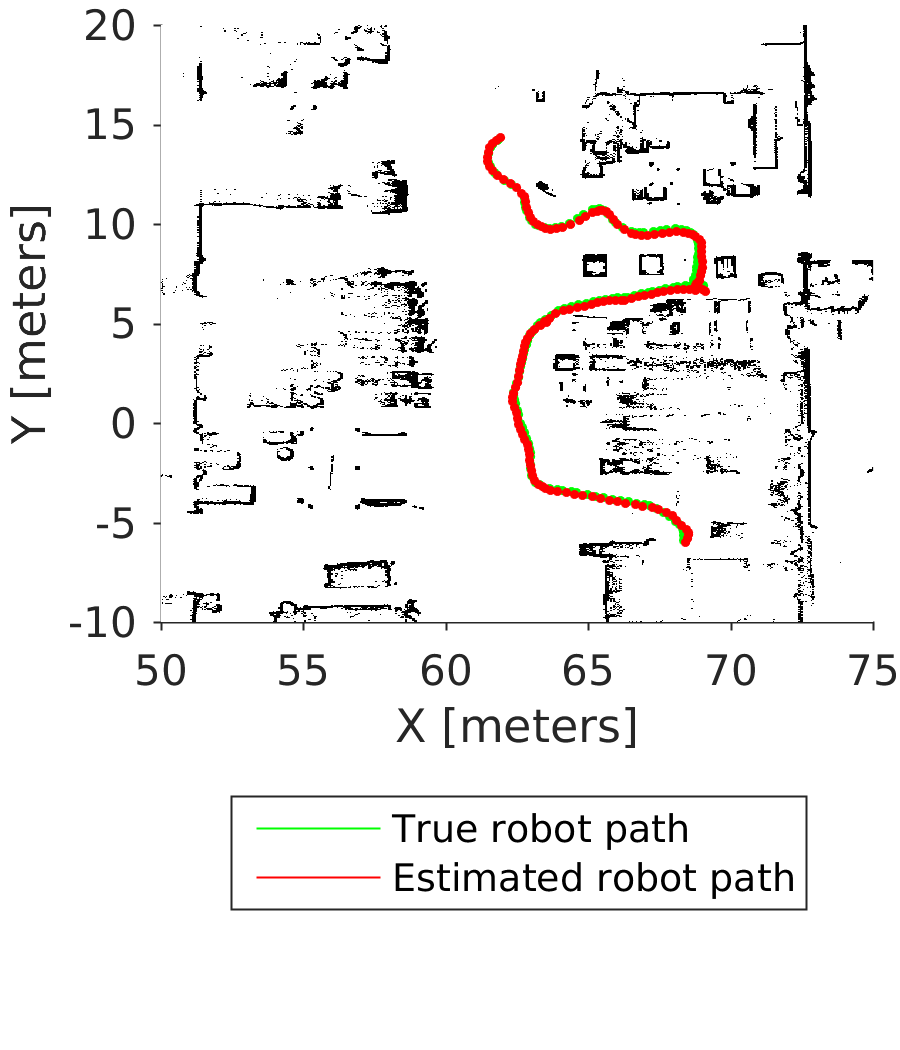
\includegraphics[width=\textwidth]{figures/static_mapping/simulated_robot_estimate_total}
		\caption{World represenation}
		\label{fig:simulated_robot_estimate_total}
	\end{subfigure}
	~ %add desired spacing between images, e. g. ~, \quad, \qquad, \hfill etc. 
	%(or a blank line to force the subfigure onto a new line)
	\begin{subfigure}[b]{0.45\textwidth}
		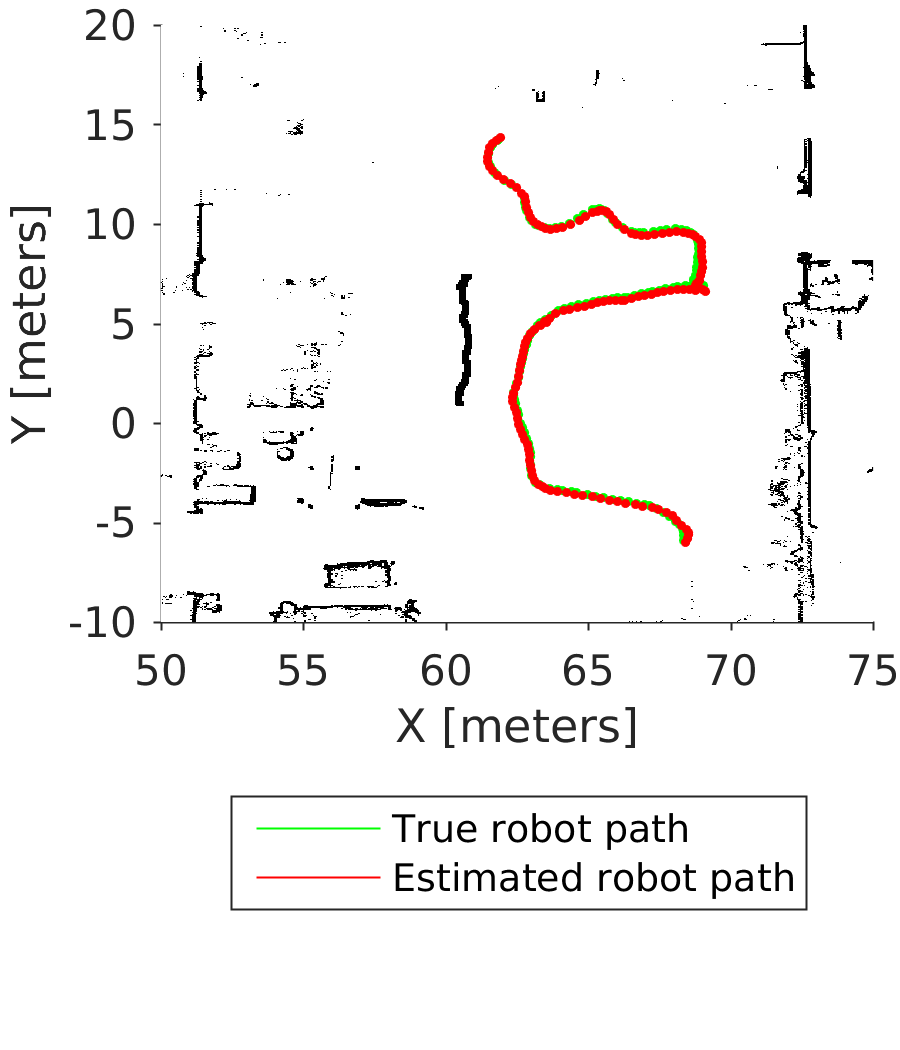
\includegraphics[width=\textwidth]{figures/static_mapping/simulated_robot_estimate_total_edited}
		\caption{Map used by AMCL}
		\label{fig:simulated_robot_estimate_total_edited}
	\end{subfigure}
	\caption{Simulation of a MIR robot moving with imprecise location.}
	\label{fig:simulated_location_error}
\end{figure}
